\section{Anwendungsfall-Modell}

"`Ein Anwendungsfall ist eine Abstraktion, die alle m�glichen Szenarien beschreiibt, die die beschriebene Funktionalit�t enthalten."'\cite[S. 76]{Bruegge_2004}\\
% Ein Szenario ist eine Instanz eines Anwendungsfalls; wenn wir diesen Anwendungsfall identifizieren, haben wir damit
% alle m�glichen Szenarien f�r eine gegebene Funktionalit�t.\cite[S. 160]{Bruegge_2004}

Anhand der in Abschnitt \ref{section:Scenarios} beschriebenen Szenarien wurden die Anwendungsf�lle identifiziert, die
zeigen, wie die Anwender mit dem System interagieren. In diesem Abschnitt wird das Anwendungsfall-Modell dargestellt und
die einzelnen Anwendungsf�lle erkl�rt. Ein vollst�ndiger Flow-of-Events zu jedem Anwendungsfall findet sich im Anhang.
Abbildung \ref{figure:usecases} gibt einen �berblick �ber die Anwendungsf�lle aus Sicht des einzigen Akteurs, des Spielers.

\begin{figure}[htbp]
\centering
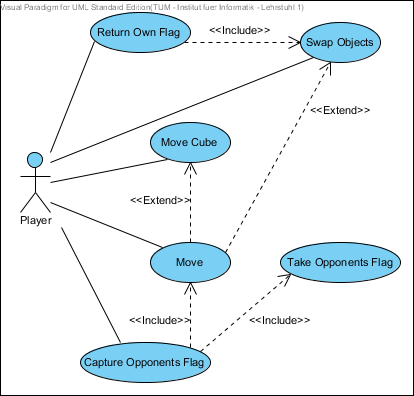
\includegraphics[width=0.8\textwidth]{images/use_cases}
\caption[Anwendungsfall-Diagramm]{Anwendungsfall-Diagramm}
\label{figure:usecases}
\end{figure}

\subsection{Cube bewegen}

\subsection{Bewegen}

\subsection{Einen Punkt erzielen}

\subsection{Flagge nehmen}

\subsection{Objekte swappen}

\subsection{Flagge zur�ckholen}